% ~~~~~~~~~~~~~~~~~~~~~~~~~~~~~~~~~~~~~~~~~~~~~~~~~~~~~~~~~~~~~~~~~~~~~~~~~~~~~
%                                 IMPLEMENTATION
% ~~~~~~~~~~~~~~~~~~~~~~~~~~~~~~~~~~~~~~~~~~~~~~~~~~~~~~~~~~~~~~~~~~~~~~~~~~~~~
\chapter{Implementation}\label{chap:4}
  \lhead{Chapter 4. \emph{Implementation}}

\section{Game}
Game class is often implemented as a set of tools operating on provided state.
With this approach, tests can be easily designed to verify functionality.
In many cases, following methods or attributes are available:
\begin{itemize}
  \vspace*{-0.25cm}
  \setlength\itemsep{-0.15cm}

  \item initial\_state - initial state of the game
  \item is\_terminal - whether the given state is terminal
  \item valid - validates given state or action on the given state
  \item actions - list of all possible actions in the given state
  \item execute\_move - returns new state after executing given action
  \item utility - value representing how the given state is beneficial
                  for given player

  \vspace*{-0.25cm}
\end{itemize}

\noindent I consider following methods also important in Quoridor, so these are
present in my implementation:
\begin{itemize}
  \vspace*{-0.25cm}
  \setlength\itemsep{-0.15cm}

  \item undo - previous state before provided action and state
  \item shortest\_path - shortest path to goal row for the given player
  \item path\_blockers - set of wall positions that could block the given path
  \item crossing\_actions - set of invalid actions that would cross already
                            placed walls

  \vspace*{-0.25cm}
\end{itemize}

\section{State}
State should be the smallest possible representation of the game state where
it can be easily distinguished between any two different states. Mathematicaly,
state $S$ can be defined as:
\begin{equation}
  \label{eqn:state_def}
  S = (c, p_y, p_g, s_y, s_g, w)
  \vspace*{-0.20cm}
\end{equation}
Here, $c\in\{0, 1\} $ represents color of the player that should move,
$p_y,p_g\in\{0,1,...,80\}$ are pawns positions,
${s_y},{s_g} \in \{0, 1, ..., 10\}$ are counts of walls in stocks,
and set of positions of placed walls are
${w = \{\,a_i\,|\,a_i \in \{0, 1, ..., 127\}, i \in \{0, 1, ..., 20\} \}}$.
One such state in python would be:
\begin{lstlisting}
state = (0, 51, 70, 5, 9, frozenset([32, 116, 119, 59, 12, 31]))
\end{lstlisting}

However, when training ANN, it may be better to convert it to zeroes and ones.
!!! TODO !!!
% TODO: ???databazovy model tiez???


\section{Context}
For speeding up validation of the moves for agents, it turned out to be faster
to keep in memory shortest paths and invalid actions such as crossing walls.
{\lstinline{QuoridorContext}} class serves this purpose.
Also, this speeded up the decision process of heuristic and path agents.

\section{Console Game}
\begin{wrapfigure}{r}{0.5\textwidth}
  \vspace*{-2.05cm}
  \centering
  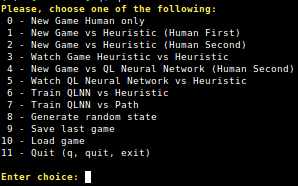
\includegraphics[width=0.48\textwidth]{main_menu.png}
  \vspace*{-0.35cm}
  \caption{main menu}
  \label{fig:main_menu}
  \vspace*{-0.70cm}
\end{wrapfigure}

Main purpose of my work was on implementation of the agent utilizing abilities
of the ANN, so the game is played and displayed in the linux terminal
(console), and so, all interactions are performed through command prompt.
To display the game properly in the terminal, it must be at least 86 characters
wide.

In the main menu (fig. \ref{fig:main_menu}), user can choose to play a game
against {\lstinline{HeuristicPlayer}} or {\lstinline{QLNNPlayer}} and also,
to watch a game played eighter by {\lstinline{HeuristicPlayer}} versus himself
or against {\lstinline{QLNNPlayer}}. Also, loading a game and saving last
played game is possible.

\begin{wrapfigure}{l}{0.5\textwidth}
  \vspace*{-0.35cm}
  \centering
  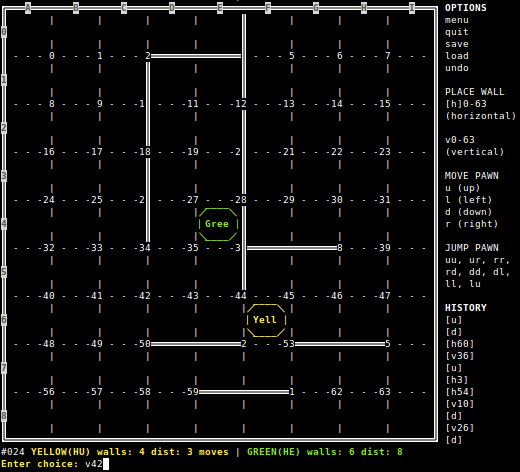
\includegraphics[width=0.49\textwidth]{game_running.png}
  \vspace*{-0.30cm}
  \caption{game running}
  \label{fig:game_running}
  \vspace*{-0.60cm}
\end{wrapfigure}

During the game (fig. \ref{fig:game_running}) to move the pawn, human players
enter first letters of words \textit{up, left, right, down}
(\textit{u, l, r, d}). To jump over opponents pawn, combination of simple
moves (\textit{uu, ul, ur, dd, dl, dr}) is used. To specify wall placement,
first letters of direction are provided (\textit{h, v}) followed by number
of the position.  For example, \textit{h3}, \textit{v24} are correctly entered
wall positions. Other options available are \textit{undo, load} or
\textit{save}.

On the right side of the game board along the options possible, user can see
some of the last moves in the HISTORY section. Below the board, there are
displayed information such as move number, wall stocks, current distances from
the goal and currently moving player.

\section{PathPlayer}
{\lstinline{PathPlayer}} is an agent that only follows shortest path to the
goal row. I have used this agent as a reference to compare number of won games
against {\lstinline{HeuristicPlayer}} and {\lstinline{QlearningNetworkPlayer}}.
User cannot choose to play against this player.

\section{HeuristicPlayer}
{\lstinline{HeuristicPlayer}}'s algorithm is following:
\begin{itemize}
  \vspace*{-0.25cm}
  \setlength\itemsep{-0.15cm}

  \item if no walls in stock, follow the shortest path
  \item if one step left to goal row, move to win
  \item if standing on the starting line, follow the shortest path
  \item if there are more than 2 possibilities to block (prolong) opponents
        path then with $60\%$ probability follow the shortest path
  \item if there are wall positions blocking opponent's path and not
        blocking it's own path and it would not cut opponent from goal row,
        place one such wall
  \item in all other cases, follow the shortest path

  \vspace*{-0.25cm}
\end{itemize}

\section{QLNNPlayer}
{\lstinline{QLNNPlayer}} evaluates every action in the current state, takes action
with maximum value and tries to play it. If move is not possible, it tries to
play next best action.

\section{Training}
To speed up the learning proccess, I have created
{\lstinline{TrainingStateGenerator}} class which provides states
to start with for the training. As a game count rises, less trivial states are
returned, until only standard initial state is used.

Each time {\lstinline{QLNNPlayer}} plays during the training game (inspired
by eq. \ref{eqn:otheloqupdate}), desired output vector $\hat{Q}_{new}(s, t)$
is a copy of current output vector $\hat{Q}(s, t)$,
where only value representing action performed by {\lstinline{QLNNPlayer}}
is updated to be eighter one of rewards $r_{t+1}$, $r_{t+2}$ or maximum of
the new q-value estimates $\displaystyle{\max_a}\hat{Q}(s', t{+}2)$
in the position, where {\lstinline{QLNNPlayer}} is on the move again.

In the training, {\lstinline{QLNNPlayer}} has probability of
playing random move decreasing over time, so that there is a chance to explore
and find better moves.

Function {\lstinline{handle_training}} running the training along with
{\lstinline{TrainingStateGenerator}} and {\lstinline{TRAINING_STATES}}
resides in module {\lstinline{quoridor.ai.training}}. It is started through
the game menu and it is possible to run training against
{\lstinline{PathPlayer}} or {\lstinline{HeuristicPlayer}}.
